\begin{figure}
    \center
    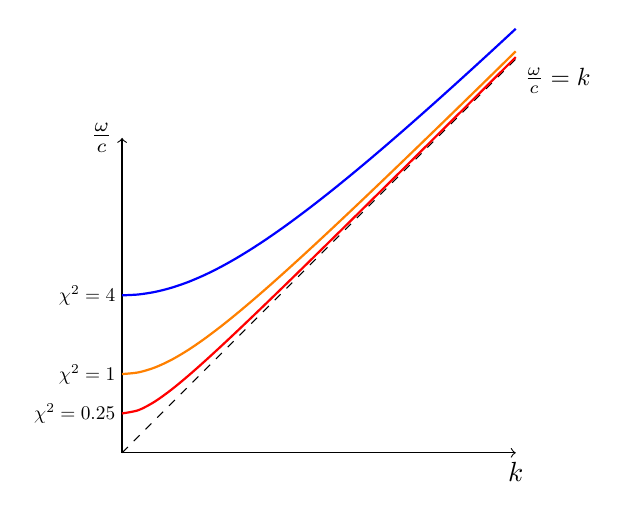
\begin{tikzpicture}
        
        \draw[->] (0,0) -- (0,4) node[left] {$ \frac{\omega}{c} $};
        \draw[->] (0,0) -- (5,0) node[below] {$ k $};

        \draw[dashed, domain = 0:5, variable = \x] plot ({\x}, {\x}) node[below right, scale = 0.9] {$ \frac{\omega}{c} = k $};
        % parametro

        \def\a{1}
        \def\b{2}
        \def\c{0.5}        

        % iperbole y = sqrt(x^2 + a^2)
        \draw[domain=0:5,smooth,variable=\x,orange,thick]
            plot ({\x},{sqrt(\x*\x+\a*\a)});
        
        \node[ left,scale = 0.7, black] at (0,1) {$ \chi^2 = 1 $};

        \draw[domain=0:5,smooth,variable=\x,blue,thick]
            plot ({\x},{sqrt(\x*\x+\b*\b)});
        
        \node[ left,scale = 0.7, black] at (0,2) {$ \chi^2 = 4 $};
        
        \draw[domain=0:5,smooth,variable=\x,red,thick]
            plot ({\x},{sqrt(\x*\x+\c*\c)});
        
        \node[ left,scale = 0.7, black] at (0,0.5) {$ \chi^2 = 0.25 $};

    \end{tikzpicture}
    \caption{Grafico delle relazioni di dispersione per vari valori di $ \chi^2 $.}
    \label{figure:_linea_luce}
\end{figure}